\chapter{Introducción}\label{cha:introduccion}

\section{Presentación del Documento}

El presente informe describe el proyecto de desarrollo Gestión de repositorios semánticos compatible con el estándar \acrshort{oaipmh}, un aplicativo que pretende extender a \acrshort{labman}, el \acrlong{dms} de los grupos de Internet y Telecomunicaciones de DeustoTech, detallando tanto los objetivos que se pretenden alcanzar con el proyecto, como las fases, actividades y recursos necesarios para llevarlo a cabo.

El contenido de este documento se estructura en torno a los siguientes productos:

\begin{itemize}
	\item \textbf{Definición de proyecto:}
		
	Establecimiento del objetivo fundamental del proyecto, especificando cuáles son los aspectos funcionales que lo comprenden y cuáles son los que quedan excluidos.
	
	\item \textbf{Producto final:}
		
	Especificación de la solución elegida que va a construir el proyecto en cuestión.
	
	\item \textbf{Descripción de la realización:}

	Realización y definición de las diferentes actividades cuyo desarrollo va a permitir la realización y consecución del objetivo del proyecto.

	\item \textbf{Organización:}
	
	Definición del equipo de trabajo que desarrollará el proyecto, así como su estructura organizativa, sistema de gestión y seguimiento del trabajo.

	\item \textbf{Condiciones de ejecución:}

	Definición del entorno de trabajo, de los criterios sobre los que se van a realizar las sucesivas recepciones, así como el tratamiento que se va a establecer para aquellos casos que puedan ser considerados como modificaciones o mejoras en el planteamiento inicial del proyecto.

	\item \textbf{Planificación:}
	Estimación de cargas y duración de las diferentes actividades del proyecto, así como su asignación a los diferentes miembros del equipo y su planificación en el tiempo.

	\item \textbf{Valoración económica:}
	Determinación del valor correspondiente a este proyecto, de los hitos de facturación y de la forma de pago.
\end{itemize}

\section{Introducción a LabMan}

Es este apartado se realiza una breve introducción a \acrfull{labman}, el \acrlong{dms} de MoreLab, el grupo de investigación formado por los equipos de Internet y Telecomunicaciones de DeustoTech y en el que se basa este proyecto.

\begin{figure}[!htp]
	\centering
	
\includegraphics[scale=0.15]{fig/morelab-logo}
	\caption{Logo de MORELab}
\end{figure}

Gestionar la información no siempre es una tarea trivial y más aún cuando hay que tratar con los datos que componen varias entidades como pueden ser los proyectos, investigadores, publicaciones, eventos, etc. dentro del ámbito de la investigación. La mayoría de los grupos de investigación utilizan sistemas de gestión de contenido tales como Joomla!\cite{joomla}, WordPress\cite{wordpress} o Drupal\cite{drupal} para exponer sus datos. Sin embargo, para extraer la información de estos \acrshortpl{cms} se requieren herramientas externas para llevar a cabo técnicas de análisis de datos. 
Para hacer uso de estas herramientas normalmente hace falta generar documentos adicionales, tales como \acrshort{csv}, hojas de cálculo, ficheros de texto, generado información redundante, que provoca dificultades a la hora de actualizar los datos y la calidad de los mismos. Esta situación empeora cuando además se disponen de distintas fuentes para la obtención de información, como pueden ser las paginas web personales de los investigadores en los que se muestran sus logros a lo largo de su carrera, la información financiera gestionada por su propio departamento, etc.

\begin{figure}[!htp]
	\centering
	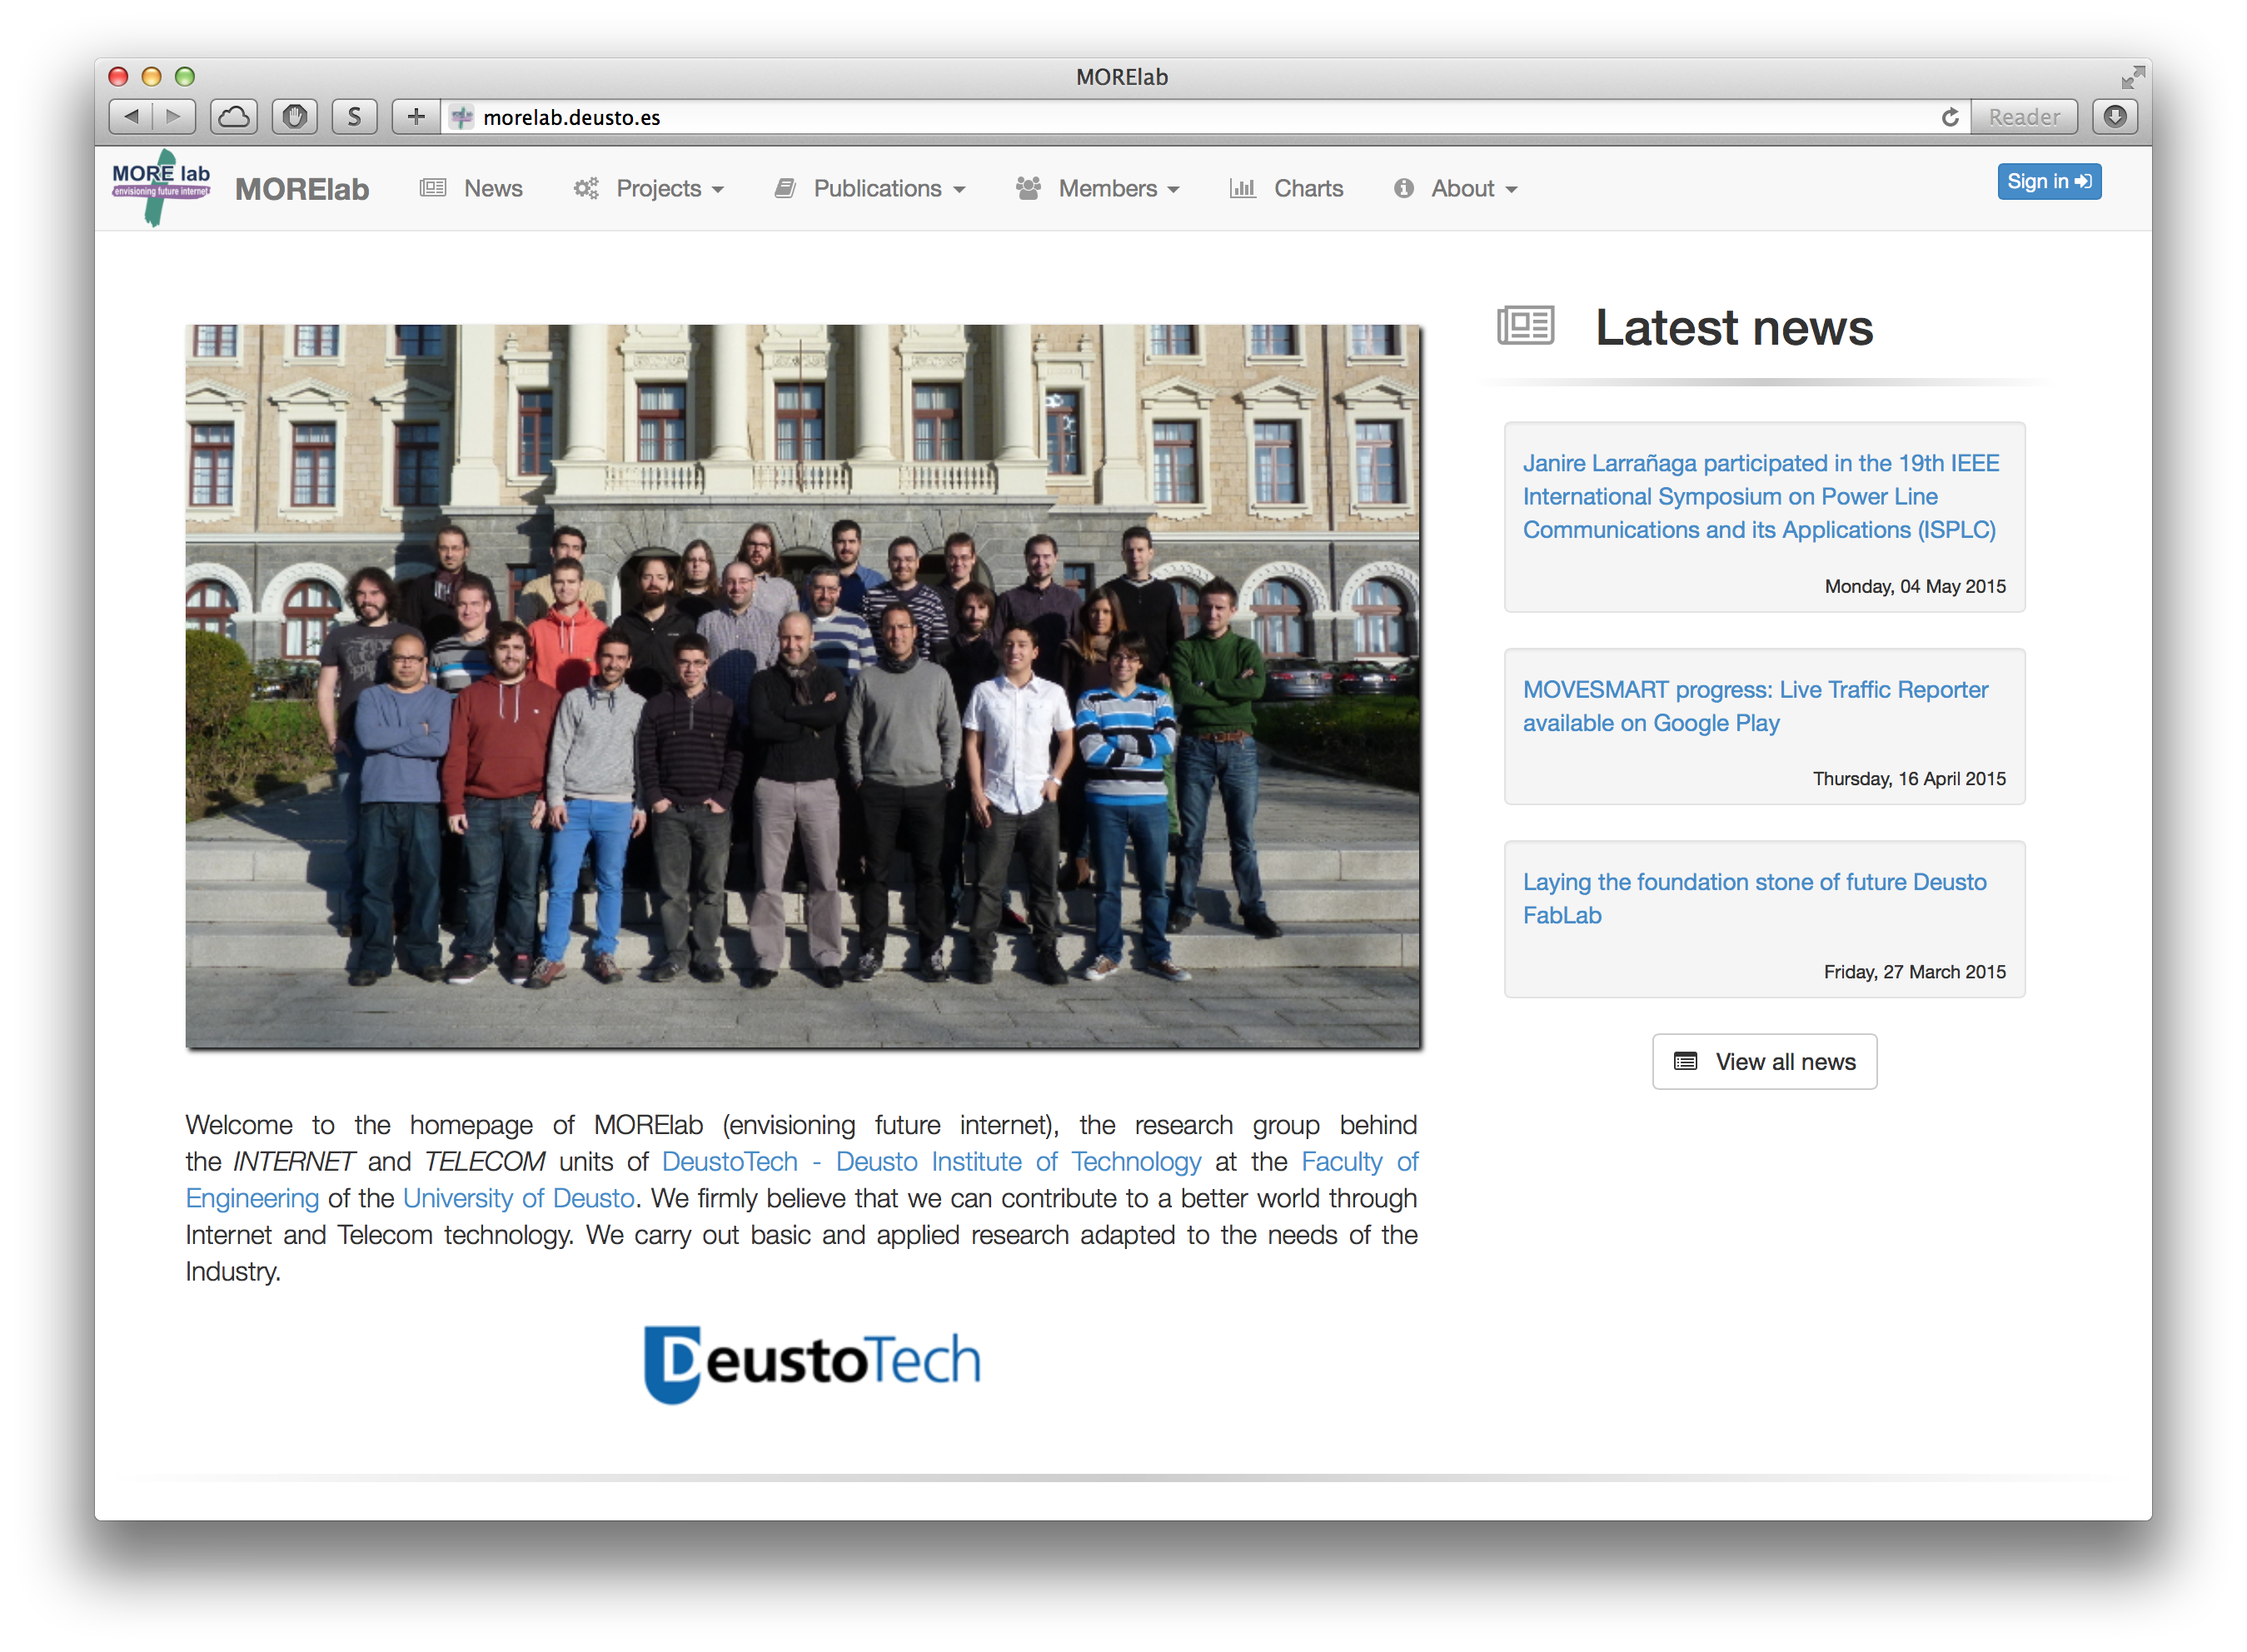
\includegraphics[scale=0.13]{fig/labman-homepage}
	\caption{Página de inicio de \acrshort{labman} con el equipo}
\end{figure}

Del esfuerzo para gestionar la información grupo de investigación de MoreLab nace \acrshort{labman}, una aplicación desarrollada en Python\cite{Python} por medio del framework para desarrollo web Django\cite{Django} y que sustituye a la antigua solución Joomla! para la publicación de los datos sobre las publicaciones en \acrshortpl{rdf}\cite{RDF}. Su principal objetivo es gestionar todo este tipo información, diferenciadose de otros \acrshortpl{cms} por apostar por la exposición de los datos como \acrlong{lod}\cite{linkeddata}, disponible por todos sin restricción de derechos de \textit{copyrights} o patentes.

Mediante el uso de los datos enlazados se es posible identificar cada entidad por medio de una \acrshort{uri}, permitiendo la creación de relaciones entre distintas instancias, lo que deriva en la posibilidad de descubrir patrones dentro de un set de datos.



\cite{pena_visual_2014}

\section{Motivación}

DeustoTech cree que es posible contribuir a un mundo mejor mediante el uso de las tecnologías de Internet y Telecomunicaciones.

Como resultado de este pensamiento nació \acrshort{labman}, un sistema de gestión de grupos de investigación. Esta aplicación web tiene como objetivo gestionar toda la información referente a los investigadores, proyectos y publicaciones de un grupo relacionada entre si. Permite generar diversas gráficas que permiten analizar de forma rápida la evolución y desempeño del grupo de investigación.

Este aplicativo es un claro ejemplo de una web de datos de nueva generación de portales web, dónde no solo se exportan documentos, sino que habilita la exportación datos y \acrshortpl{api}, que tienen como propósito facilitar la explotación de datos.

Aunque es capaz de exportar esta información semántica, todavía se ve la necesidad de que el sistema colabore con sistemas imperantes en la industria para el intercambio de información de recursos académicos y científicos.
Es por ello que se desea dar soporte a \acrshort{oai}, mediante la implementación de su protocolo \acrlong{oaipmh}, más comúnmente conocido por sus siglas \acrshort{oaipmh}, para poder comunicarse y dar servicio a soluciones del sector que apostaron por esta tecnología, favoreciendo por otra parte una mayor explotación de la información.

Así mismo se desea fomentar accesibilidad a dichos recursos, teniendo en especial consideración a aquellos usuarios que no disponen de conocimientos informáticos, por medio de un cliente web que sirva tanto de buscador como de filtrador.

Esta accesibilidad se garantizará mediante un estudio exhaustivo de los distintas formas en las que se pueden disponer los formularios y de cómo el usuario interactúa con ellos, teniendo como resultado una interfaz de usuario que asegura una experiencia intuitiva.
